%%%%%%%%%%%%%%%%%%%%%%%%%%%%%%%%%%%%%%%%%%%%%%%%%%%%%%%%%%%%%%%%%%%%%
% LaTeX Template: Project Titlepage Modified (v 0.1) by rcx
%
% Original Source: http://www.howtotex.com
% Date: February 2014
% 
% This is a title page template which be used for articles & reports.
% 
% This is the modified version of the original Latex template from
% aforementioned website.
% 
%%%%%%%%%%%%%%%%%%%%%%%%%%%%%%%%%%%%%%%%%%%%%%%%%%%%%%%%%%%%%%%%%%%%%%

\documentclass[12pt]{report}
\usepackage[a4paper]{geometry}
\usepackage[myheadings]{fullpage}
\usepackage{fancyhdr}
\usepackage{lastpage}
\usepackage{graphicx, wrapfig, subcaption, setspace, booktabs}
\usepackage[T1]{fontenc}
\usepackage[font=small, labelfont=bf]{caption}
\usepackage{fourier}
\usepackage[protrusion=true, expansion=true]{microtype}
\usepackage[english]{babel}
\usepackage{sectsty}
\usepackage{url, lipsum}
\usepackage{float}
\usepackage[switch, modulo]{lineno}
\usepackage{amsmath} % for 'bmatrix' environment
\usepackage{color}
\usepackage{algorithm}
\usepackage[noend]{algpseudocode}
\usepackage{verbatim}
\usepackage{minted}
\usepackage[normalem]{ulem}
\useunder{\uline}{\ul}{}


\mathchardef\mhyphen="2D
\newcommand{\HRule}[1]{\rule{\linewidth}{#1}}
\onehalfspacing
\setcounter{tocdepth}{5}
\setcounter{secnumdepth}{5}

\def\doubleunderline#1{\underline{\underline{#1}}}

%-------------------------------------------------------------------------------
% HEADER & FOOTER
%-------------------------------------------------------------------------------
\pagestyle{fancy}
\fancyhf{}
\setlength\headheight{15pt}
\fancyhead[L]{Oisin Wellesley-Miller}
\fancyhead[R]{Exeter Mathematics School}
\fancyfoot[R]{Page \thepage\ of \pageref{LastPage}}
%-------------------------------------------------------------------------------
% TITLE PAGE
%-------------------------------------------------------------------------------

\begin{document}

\title{ \normalsize \textsc{Exeter Mathematics School}
		\\ [2.0cm]
		\HRule{0.5pt} \\
		\LARGE \textbf{\uppercase{Audio to MIDI conversion}}
		\HRule{2pt} \\ [0.5cm]
		\normalsize \uppercase{A-Level Computer Science NEA} \\
		\today \vspace*{5\baselineskip}}

\date{}

\author{
		Oisin Wellesley-Miller }

\maketitle
\tableofcontents
\newpage
%-------------------------------------------------------------------------------
% Section title formatting
\sectionfont{\scshape}
%-------------------------------------------------------------------------------

%-------------------------------------------------------------------------------
% BODY
%-------------------------------------------------------------------------------
% USE CASE: The music is not uploaded to 3rd party so confidential music is not shared and no issues with copyright ect is run into

\section*{Analysis}
\addcontentsline{toc}{section}{Analysis}
% Overview
% Research
% - Wav and MIDI
% - DFT and FFT
% - Existing Solutions
% End User
% Solution
% Objectives
% Limitations
% Extentions

\subsection*{Overview}
\addcontentsline{toc}{subsection}{Overview}
The Fast Fourier Transform (FFT) is one of the most important mathematical algorithms that exists and its applications have shaped our modern lives. In my project I will be using a Fast Fourier Transform in order to convert a recording of someone playing a piano into a MIDI file of the same recording. \\
A MIDI (.mid) file is a file format that is commonly used to store and edit compositions of music digitally. It stores which note is being played at which time and for how long, allowing the piece to be built up of the different notes being played at a time. On the other hand, a wave file (.wav) instead stores the magnitude of the wave it can hear through time. When writing and producing music it is often more beneficial to work with midi files as they allow for editing, as the characteristics of individual notes and sounds can be changed. Converting a midi file into a wave file is a simple task, as it only needs to be played through a midi synthesizer and a recording made. However converting in the other direction is a lot more complex, as instead of combining multiple sounds together they instead need to be separated from one another. If this conversion was able to be done easily, then it would be easier for people to edit music without having to use expensive midi instruments to produce the midi files.\\
In order to take this in and convert it to the note (or notes) being played at a time a Discrete Fourier Transform will have to be performed on the data. This will convert the amplitude over time graph to a graph that shows how much of each frequency is present in a sample. By analysing many samples over the course of the recording my program will be able to determine the note being played and write this to the MIDI file.

\subsection*{Research}
\addcontentsline{toc}{subsection}{Research}
My research was split into 3 different topics: The mathematics and algorithms behind the Fourier Transform, research into the exact format of MIDI and wave files and research into existing solutions that perform this conversion.
 \newline
 \newline
During this research phase of my project I found information on a wide variety of sites, here is list of many that I used (All links accessed September 2018):\\
\begin{itemize}
    \color{blue}
    \item https://en.wikipedia.org/wiki/MIDI\#MIDI\_files
    \item https://en.wikipedia.org/wiki/WAV
    \item http://www.ccarh.org/courses/253/handout/vlv/
    \item https://youtu.be/qeb4Dc3gpdo
    \item https://youtu.be/\_7U8hzBNyxk
    \item https://en.wikipedia.org/wiki/Fourier\_transform
    \item https://www.ams.org/journals/mcom/1965-19-090/S0025-5718-1965-0178586-1/home.html
    \item https://www.recordingblogs.com/wiki/musical-instrument-digital-interface-midi
    \item https://www.recordingblogs.com/wiki/orinj-working-with-midi-files
    \item https://www.avrfreaks.net/forum/how-decode-wav-fileson
    \item https://www.midi.org/specifications/item/table-1-summary-of-midi-message
    \item https://stackoverflow.com/questions/13039846/what-do-the-bytes-in-a-wav-file-represent
    \item https://en.wikipedia.org/wiki/Piano\_key\_frequencies
\end{itemize}

\subsubsection*{WAVE and MIDI}
\addcontentsline{toc}{subsubsection}{WAVE and MIDI}

The end result of this project will be a program capable of reading in a .wav file that contains a recording of somebody playing a piece on a piano, process it and then return a .mid file the same piece of piano music. In order to do this I will need to understand exactly how both the .wav and .mid file formats work.

For most applications a wave file is a perfectly adequate way of storing audio data, however its downfalls come in file size and editabilty. Because of the large amount of data they store they are slow to edit as many different changes must be made to the file to represent a small change in how the sound sounds. Midi on the other hand is extremely easy to edit and tweak as this format only stores what note is being played when. The problem I am trying to solve is turning a recording of music in wave format into midi format in order to edit the music.

So first of all what are MIDI and wave files and how are they different? Well, both are methods of digitally representing sound loosely based on the RIFF format but the similarities end there. 

Wave (.wav or .wave) files directly store the uncompressed audio wave that they represent so that a computer may easily reconstruct it. They do this by taking a number of samples through time of what a microphone can hear, then storing these values one after another in a file. The most common sampling rate for audio is 44.1KHz (44100 samples a second) as this can be used accurately reconstruct a sound wave to the standards of human hearing, as shown by Nyquist's Theorem as the human hearing usually goes up to around 20KHz. This way of storing audio results in a very faithful representation of the original sound, but at the cost of very large file sizes.

MIDI (.mid) files represent audio in a very different way. They are specialised to store music and instead of representing the sound wave at a particular time they instead store a series of MIDI commands. These commands represent what instrument is playing what note at what time at what volume. This allows for MIDI files to be very easily edited and tweaked as well as allowing them to have incredibly small file sizes, as each command is only a few bytes. However in order to play MIDI files, the machine playing them must have a large number of samples of different instruments playing different notes stored on it so that it knows what to play for each MIDI command. This means that the final quality of the sound being played depends entirely on the device playing the file and not on how the file was recorded as is the case for most other audio formats.

Once the data is read from the wave file and a Fourier Transform performed, the note being played at a particular time must be determined by comparing the found frequencies to the known frequencies of different notes. Once this is done and the start and stop time of the note is known, it can be converted to a MIDI start note command and a MIDI stop note command that can then be written to the MIDI file with the correct delta times. This delta time is a variable length value that stores the time that should be waited before processing the next command in sequence.

\subsubsection*{DFT and FFT}
\addcontentsline{toc}{subsubsection}{DFT and FFT}

To begin my research I looked into the Fourier Transform. This is a mathematical transform capable of splitting complicated periodic functions into their components for easy analysis. A very common application of this is to split a wave through time into it's component frequencies, which will be how I plan to use it in this project. There are many other applications of this however, such as in audio editing, image editing, compression and even in our mobile phones. For this project I will need to determine the frequency of a note (or notes) being played at a particular time, so I will need to split the sound wave stored in the .wav file into its frequencies with a Fourier Transform and then analyse these before writing them to the .mid file.

\begin{figure}[!ht]
	\centering
	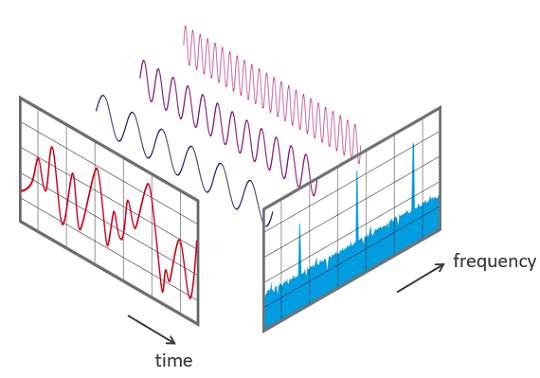
\includegraphics[width=0.5\textwidth]{fourier.png}
	\caption{View of a signal through both frequency and time domains \cite{FFT}}
	\centering
	\label{label:fft_diagram}
\end{figure}

The general Fourier Transform of a function $f(x)$ if usually defined as $\hat{f}(\xi)$, as shown by equation \ref{eq:Fourier_Transform}. In this case $x$ would represent time and $\xi$ represents the frequency of the wave. 

\begin{equation}
    \hat{f}(\xi) = \int_{-\infty}^{\infty}f(x) \cdot e^{-2 \pi i x \xi} dx 
    \label{eq:Fourier_Transform}
\end{equation}

%The Fourier Transform

However, the above version of the Fourier Transform only applies to continuous functions. In order to perform a Fourier Transform on a series of data, for example the amplitudes stored in a .wav file, instead a Discrete Fourier Transform (DFT) must be used. This will have the same effect as a Fourier Transform but can be performed on a series of equally spaced samples instead of a function. In order to transform a series of N complex numbers $\{x_n\} := x_1, x_2,..., x_{n-1}$ into their Fourier Transform $\{X_n\} := X_1, X_2,..., X_{n-1}$ the following function can be used:

\begin{equation}
    X_k = \sum_{n=0}^{N-1} x_n \cdot e^{-2 \pi i k n / N}
    \label{eq:Discrete_Fourier_Transform}
\end{equation}

%\begin{equation}
%    x_n = \frac{1}{N} \sum_{k=0}^{N-1} X_k \cdot e^{i 2 \pi k n / N}
%    \label{eq:Discrete_Inverse_Fourier_Transform}
%\end{equation}

When actually computed, the DFT is often implemented using matrices to improve efficiency. The samples being transformed are put into a vector and transformation matrix is then constructed, when multiplied together they then result in an output vector of frequencies as shown below in figure \ref{eq:Discrete_Fourier_Transform_Matrix}. When performed in this way the computational complexity of the is $O (n^2)$. What this means is that in order to transform $n$ samples, $n^2$ calcula'tions must be performed and 2x increase in the number of samples will result in a 4x increase in the number of calculations. This is quite good as far as efficiency goes however it can be improved through the use of a different algorithm for computing the DFT.

\begin{align*}
    Let \quad \omega_{N} = e^{-2 \pi i / N} \
\end{align*}

\begin{equation}
    \begin{bmatrix} 
        \hat{f}_{0} \\
        \hat{f}_{1} \\
        \vdots  \\
        \hat{f}_{(N-1)}
    \end{bmatrix}
    =
    \begin{bmatrix} 
    1 & 1 & \dots  & 1\\
    1 & \omega_N  & \dots & \omega_N^{(N-1)}\\
    \vdots & \vdots & \ddots & \vdots\\
    1 & \omega_N^{(N-1)} & \dots &  \omega_N^{(N-1)^2}
    \end{bmatrix}
    \begin{bmatrix} 
        f_{0} \\
        f_{1} \\
        \vdots  \\
        f_{(N-1)}
    \end{bmatrix}
    \label{eq:Discrete_Fourier_Transform_Matrix}
\end{equation}

Instead a Fast Fourier Transform (FFT) can be used which will improve the computational complexity to $O(n\log{n})$. This FFT algorithm is one of the most important algorithms ever developed and it is ubiquitous in our modern lives. The FFT was first developed in 1805 by Carl Friedrich Gauss in an unpublished manuscript\cite{gauss}, however it was not until 1965 when it was independently rediscovered by Cooley and Tukey\cite{cooley} that it saw widespread usage. The main idea behind the algorithm is work with a number of samples equal to a power of two. This allows for the Fourier Transform matrix $\doubleunderline{\mathbb{F}}$ to be split into separate operations for the odd and even indexed samples, and then split again multiple times. The dramatically improves efficiency as many values in the matrices are replaced with zeros meaning that less computations have to be carried out. This process can be seen below:

\begin{align*}
    \underline{\hat{X}} = \doubleunderline{\mathbb{F}}_{2^p} \mkern6mu \underline{X}
\end{align*}

\begin{align*}
    \underline{\hat{X}} =
    \begin{bmatrix} 
        I & -D \\
        I & -D
    \end{bmatrix}
    \begin{bmatrix} 
        F_{2^{p-1}} & 0 \\
        0 & F_{2^{p-1}}
    \end{bmatrix}
    \begin{bmatrix} 
        \underline{X}_{even} \\
        \underline{X}_{odd}
    \end{bmatrix}
\end{align*}

\begin{align*}
    Where \quad D = 
    \begin{bmatrix} 
    1 & 0 & 0 & \dots & 0\\
    0 & \omega_N  & 0 & \dots & \vdots\\
    0 & 0 & \omega_N^2 & \ddots & \vdots\\
    \vdots & \vdots & \ddots & \ddots & 0\\
    0 & \dots & \dots & 0 &  \omega_N^{2^{p}-1}
    \end{bmatrix}
\end{align*}

\begin{align*}
    F_{2^{p}} =
    \begin{bmatrix} 
        F_{2^{p-1}} & 0 \\
        0 & F_{2^{p-1}}
    \end{bmatrix}
\end{align*}

With this FFT algorithm each time $F_{2^{p}}$ is broken down, the efficiency increase by a factor of two, as half of the resulting matrix becomes zeros.

Interestingly even if the number of samples is not exactly a power of 2, it is still dramatically more efficient to pad the samples vector with zeros until a power of two is reached and then perform a FFT than it would be to perform a DFT.

\subsubsection*{Existing Solutions}
\addcontentsline{toc}{subsubsection}{Existing Solutions}
%https://www.ofoct.com/audio-converter/convert-wav-or-mp3-ogg-aac-wma-to-midi.html
\underline{Bear File Converter}\\
\textcolor{blue}{https://www.ofoct.com/audio-converter/convert-wav-or-mp3-ogg-aac-wma-to-midi.html}\\
The first solution I found was this website, which allows the user to convert one of a variety (WAV, MP3, OGG, AAC, WMA) of file formats into a MIDI file. Most of this website is covered in advertisements, but a screenshot of the actual conversion UI can be seen below.

\begin{figure}[H]
	\centering
	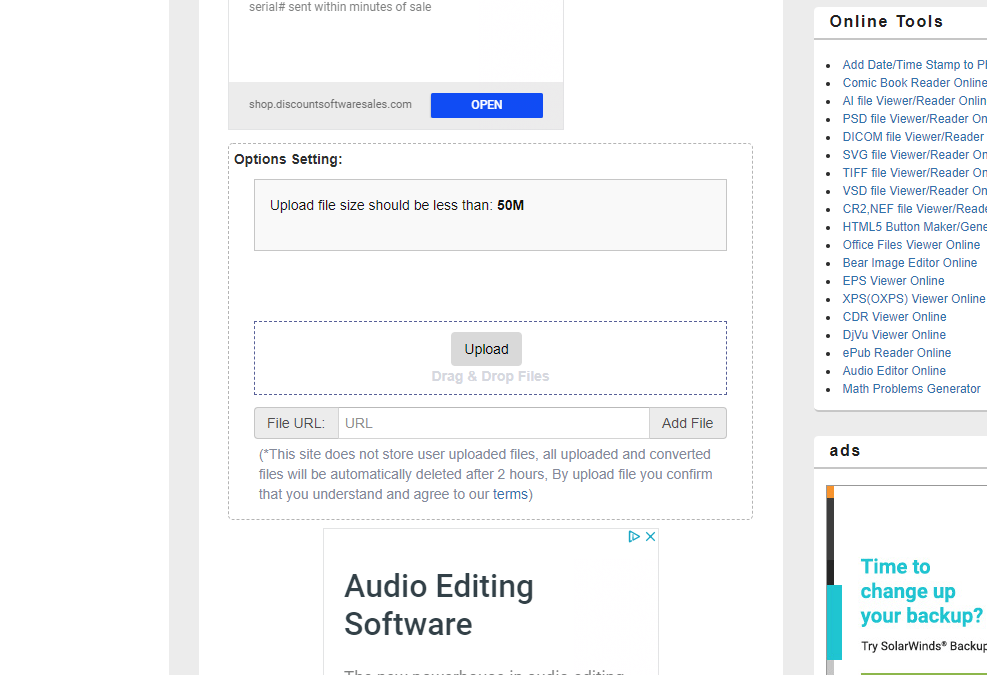
\includegraphics[width=0.5\textwidth]{site1.PNG}
	\caption{The Bear File Converter}
	\centering
	\label{label:bear_site1}
\end{figure}

The website is very simple to use once the options are found on the page, there is an input box to add the URL of web-hosted file or to upload a local file. Once a file has been added options will then appear to add additional files for a batch conversion, convert all added files, to download all converted files or to download an individual file.

\begin{figure}[H]
	\centering
	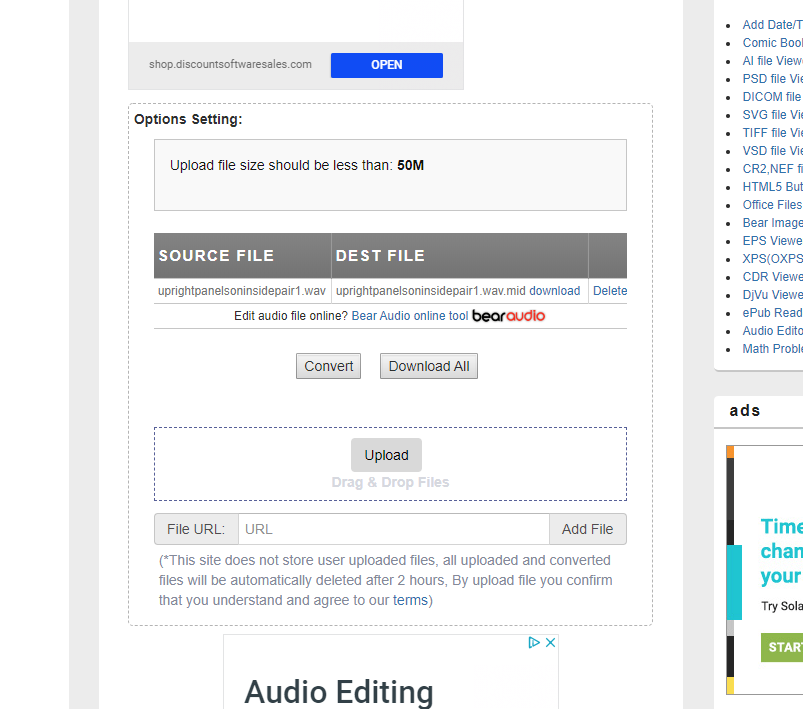
\includegraphics[width=0.4\textwidth]{site2.PNG}
	\caption{Bear File Converter Options}
	\centering
	\label{label:bear_site2}
\end{figure}

Once the converted MIDI files are downloaded they can then be easily played by a MIDI sequencer. This site has a very easy to use interface (once you find it amongst the ads) that makes it very simple to convert a file, however the quality of the final MIDI file varies significantly with the song being converted. Some pieces convert almost flawlessly, with only a few minor glitches, whereas the results of other sound like someone randomly bashing the keys of a piano. From the testing I have done it seems the more chords being played at once and the faster the tempo of the music the more likely it is to "fail" in the conversion, though overall this solution is very robust.\\

I was unable to test any other existing solutions during my research as the only other solutions I could find were part of expensive software packages (such as Ableton\cite{Ableton}, Widisoft\cite{Widisoft}, Wavesum\cite{Wavesum})

\subsection*{End User}
\addcontentsline{toc}{subsection}{End User}
In order to determine the exact features that that my end user will find important I conducted an interview with them, I have included the questions and their responses below:

\begin{itemize}
\item Question: What are you going to be using this application for?\\
"I need this program to help me when I am writing music, I like to try out different melodies that I hear on TV or the internet ect to experiment. The problem is my pitch is not very good so I struggle to work out what notes are playing, hopefully this program should help me with this. I'd also like to be able to edit and see the code myself, I don't want something that runs on a server somewhere I'd like to know exactly what is happening to the music that goes through it."
\item Question: Are there any particular features that will be important?\\ 
"I need the ability to run this on a multitude of devices, such as my desktop that runs Windows and my laptop that runs Linux. I also would like it to be able to identify different chords, but this isn't that important for me."
\item Question: How important is the speed at which it works?\\ 
"I'd like it to be relatively fast, but I don't mind too much if it isn't as I can be working on other ideas when I wait for it to complete."
\item Question: Is a GUI an important feature?\\ 
"It would be nice to see but not essential, I use some other command line tools so I would be used to working without a GUI."
\item Question: How important is the accuracy?\\ "I think getting the different pitches correct is important, I don't mind about the timings being exactly correct as I can more easily edit these from the midi file and what I can hear from the original. Obviously if it get's it completely correct that would be best."
\end{itemize}

From this I have determined that the end user for this project is a musician who needs a simple solution to music transcription, current .wav to .mid are either part of expensive software packages, are sketchy links on file hosting sites or require uploading the file to a 3rd party server. My client wants a solution that will combat all three of these issues: It must be available to them for free, and not require the installation of an .exe from a potentially unsafe source and be use-able without uploading their new music to a 3rd party. As part of their requirements they need the program to be able to run on both Windows and Linux, be easy to use and quite quick to process.





\subsection*{Solution}
\addcontentsline{toc}{subsection}{Solution}
My solution will be a GUI based program capable of performing the file conversion of a Wave file to a MIDI file through the use of a Fourier Transform. I will read in a Wave file extract the sampling rate and sample data from it and store it as an object within my program. The program will then move through the file and perform multiple Fourier Transforms on different slices to build up a model of which notes are probably being played at each time. This will be calculated through the use of custom matrix classes. Once this is done, the resulting probabilities will be converted into a MIDI object that will hold the MIDI commands needed to represent the notes. Finally this will be written to a file and a success message displayed to the user.

The GUI will look something like the below image, but this is just a rough mock-up of the UI elements that are needed.

\begin{figure}[H]
	\centering
	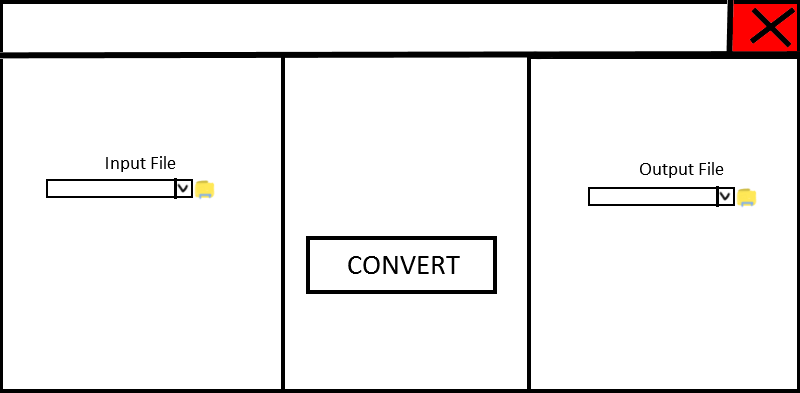
\includegraphics[width=0.6\textwidth]{mockup.png}
	\caption{GUI Mock-up}
	\centering
	\label{label:mockup}
\end{figure}

\subsection*{Objectives}
\addcontentsline{toc}{subsection}{Objectives}
\begin{enumerate}
    \item The program must be able to read the samples from a wave file into an object that represents the samples and information of the file, providing the input file is under a length of 3 minutes.
    \item The program should be able to read the amplitudes of the wave object to approximate volume.
    \item The program must be able to perform the matrix operations:
    \begin{enumerate}
        \item Addition
        \item Multiplication
        \item Slicing
        \item Concatenation
    \end{enumerate}
    \item The program must be able to correctly write the results to a midi file.
    \item The user must be able to select a wave file to convert using a GUI.
    \item The user must be able to select a wave file to convert without using a GUI.
    \item The user must receive conformation that the conversion has taken place successfully, or that an error of some kind has occured.
    \item During conversion, the user should have visual feedback in the form of a timer or progress bar to ensure the program is functioning.
    \item The program must be able to convert files that have only one note played at a time.
\end{enumerate}

\subsection*{Extensions}
\addcontentsline{toc}{subsection}{Extensions}

As an extension to the above basic functionality, some of the following features could be added to improve the program:

\begin{enumerate}
    \item The program should be able to correctly pick up on the velocity with which notes are played, relative to each other.
    \item The program could be able to convert files that have multiple notes being played at a time.
    \item The user could be able to queue the conversion on multiple files.
\end{enumerate}

\subsection*{Limitations}
\addcontentsline{toc}{subsection}{Limitations}
The limitations of this program will likely be in the conversion of wave files that are not of sufficient quality or include other instruments than a piano. These will not be able to be converted as the frequencies they contain will not correctly map to piano notes. The program may also struggle with the conversion of multiple notes being played at the same time in quick succession, as there may not be enough data to work out if a sound is more than one note or not.

\section*{Documented Design}
\addcontentsline{toc}{section}{Documented Design}
% Overview
% Algorithms
% Data structures
% Assorted diagrams

\subsection*{Preliminary Programming and Extra Research}
\addcontentsline{toc}{subsection}{Preliminary Programming and Extra Research}
Before I started work on my final solution I started by making some different test versions of my converter. For this I used the signal processing functions from Numpy instead of implementing them myself a this meant I could easily switch in and out different steps and observe the changes these made to the output without having to re-write each one each time. 
Before I could start coding anything I had to do some further research into methods that had been tried before, I began by reading through several papers on this topic \cite{spectrum} \cite{autocorrelation_transcription} \cite{pitch_detection} \cite{pitch_perception}. I found that there were several different approaches that I could try but there wasn't a know perfect method, so anything that I produce couldn't be perfect in operation. A few methods used auto-correlation whereas others instead just used the FFT and some post-processing so I decided I would need to try out both and see what I could get working.
To begin with I tried to determine the pitch at a time using a process called auto-correlation, this involved taking a sample and offsetting it with itself and computing the Pearson correlation coefficient and then storing them into a result list. This process can be sped up by using Fourier transforms by utilising the Weiner-Khinchin Theorem\cite{w_k}.
After implementing this I found that it was very slow and did not give results that were as clear as just using a FFT. Although theoretically this use of autocorrelation should be able to cope with chords better I did not find it as easy to extract the notes from its results, so I ended up not using this method in favour of a pure FFT approach.

Overall I believe that I should be able to match then effectiveness of the Bear file converter, however exceeding its accuracy and speed will be a very difficult task due to the complexity involved in the project I have chosen. There is no known method for transcribing files will 100\% accuracy in a reasonable compute time, but my approximation should be enough to meet the needs of my user and therefore enough for the scope of this project.

\subsection*{Overview}
\addcontentsline{toc}{subsection}{Overview}
This program will be written in Python 3.7 it provides an easy way of dealing with files and binary, as well as easy rapid prototyping. Although this may not produce a result that is as efficient to run as say Java, it will a lot easier to produce and extend. Additionally, efficiency is not an absolute priority for this project as evidenced by the answers gained from the questions in the Analysis section.

The main algorithm that my program is using is the FFT, the mathematics of which which I have briefly explained in my analysis section. This is a recursive algorithm where each step reduces the computational complexity by a factor of two. When applied to a signal through time, it will transform it into a representation of the different frequencies present as mentioned in the analysis. Once a user has selected a file to convert to midi using the GUI, the file will be read in and one track will be separated and stored into a matrix. This matrix will then be iterated over with a sliding window to determine the note at each position. This data will then be turned into midi events, sorted, and written to a midi file. This process is shown in the image overleaf (Figure 5).

\begin{figure}[H]
	\centering
	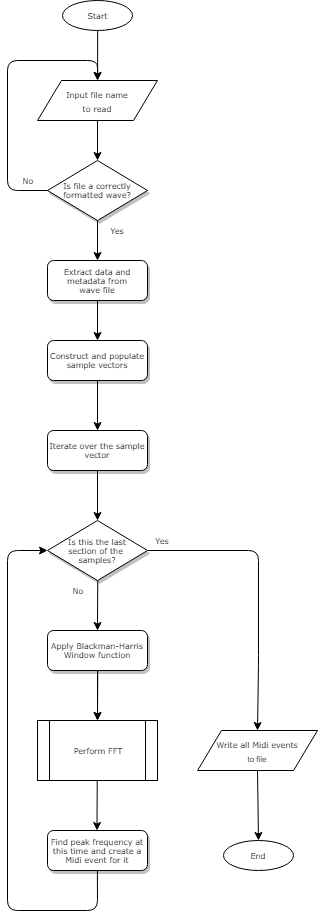
\includegraphics[width=0.5\textwidth]{flow_1.jpg}
	\caption{Program Flow}
	\centering
\end{figure}

\subsection*{Data Structures}
\addcontentsline{toc}{subsection}{Data Structures}
I have used an object orientated design structure for this project as it easily allows me to see how the functionality of different sections should interact with each other. I have tried to ensure each class completely encapsulates all of the data it need to work on and that they only interact with each other in ways that I have designed through the used of getter and setter methods. I have also used the convention of underscores to denote the attributes which should remain private to each class in order to ensure any other programmers can easily understand the structure of my code.

This section will now briefly discuss the purpose of each class and the methods that they can perform, Figure 6 shows the inheritance relationships between the different classes, along with their methods and attributes.

\begin{figure}[H]
	\centering
    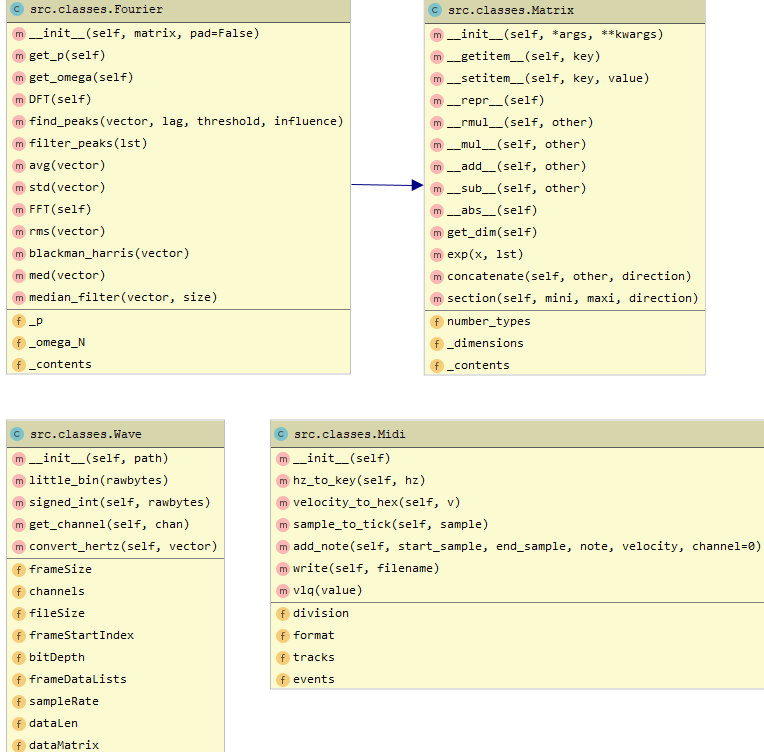
\includegraphics[width=0.85\textwidth]{class_diagrams.PNG}
	\caption{Hierarchy Chart}
	\centering
\end{figure}

\subsubsection*{Wave File}
\addcontentsline{toc}{subsubsection}{Wave File}
The wave file class deals with the initial input of a .wav file to the program. It reads in the file as binary and carefully parses the file's metadata to ensure it follows a format that the program can understand. Once the relevant information such as sample rate, filesize, number of channels and bit depth have been extracted, each different channel of audio is read and transferred into a separate column within a matrix. In order to understand the exact layout of a wave file I used a reference page \cite{Wave} from an old Stanford University website. The main information I needed was the layout of the file's header, as this would contain the metadata about the file that I would need to know in order to read in the samples. The wave file format is a subset of the RIFF file format and so consists of a file header followed by a number of data chunks, depending on the amount of data stored. This makes the job of reading the file very easy, as the needed values can be found in set locations defined in the header chunk.

\begin{figure}[H]
	\centering
	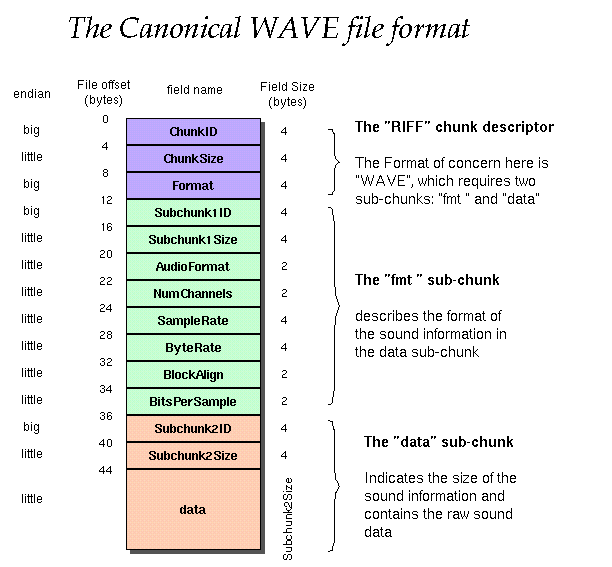
\includegraphics[width=0.75\textwidth]{wav-sound-format.png}
	\caption{Wave File Format}\label{wav_form}
	\centering
\end{figure}

When the data is needed for a conversion, the specified audio channel is then transferred to its own matrix and sent for processing. This class is quite simple in terms of functionality as it need to only read in wave files, so the only complex methods it has are to do with the conversion of the little-endian hex to signed integers.

\begin{table}[H]
\begin{tabular}{|l|l|l|}
\hline
\textbf{Function Name} & \textbf{Inputs}  & \textbf{Description}                                                                                                                                                                       \\ \hline
\_\_init\_\_           & A file path      & \begin{tabular}[c]{@{}l@{}}The Wave's constructor, loads the wave\\ file from the specified path into an object.\\ Each audio channel is stored into a \\ column in a Matrix.\end{tabular} \\ \hline
little\_bin            & Some Bytes       & \begin{tabular}[c]{@{}l@{}}Converts the provided bytes into an \\ unsigned 32 bit integer, using little endian\\ form.\end{tabular}                                                        \\ \hline
signed\_int            & Some Bytes       & \begin{tabular}[c]{@{}l@{}}This converts the bytes into a signed\\ integer, using the bit depth of the file.\end{tabular}                                                                  \\ \hline
get\_channel           & A channel number & \begin{tabular}[c]{@{}l@{}}This gets a specific channel of audio, from\\ the Matrix where they are stored.\end{tabular}                                                                    \\ \hline
convert\_hertz         & A Matrix         & \begin{tabular}[c]{@{}l@{}}This converts a Matrix from an FFT output\\ into the corresponding values in Hz.\end{tabular}                                                                   \\ \hline
\end{tabular}
\end{table}

\subsubsection*{Midi File}
\addcontentsline{toc}{subsubsection}{Midi File}
The midi file class is used to collect midi events and write them to a specified output file. It can be configured to write with different numbers of tracks and time signatures, although for this project they are set to be 1 and 96 respectively. As the conversion progresses the class will accumulate a list of midi events which it will create from a given start time, length and pitch. Once the process is finished, the events must be prepared for writing by converting their start times and lengths into note on and note off events. Since a midi file is read event by event, each note on/off event also need to be given a delta time so the interpreter/synthesizer knows how long to wait before progressing to the next event. In a midi file these delta times are stored as VLQs (Variable Length Quantity) as opposed to a traditional fixed length binary number. This means that they can use as many bytes as needed to represent an arbitrarily large number without wasting extra bits for leading 0s when storing smaller numbers. However, because each number is represented with a different number of bits, this makes reading in midi files a difficult task as special care must be taken to separate the different values from each other. Luckily for this project only the ability to write midi files is required, so this simplifies things considerably. 

The main functions of this class are type conversion, for example the Hz to midi note formula, sample to tick and variable length quantities. The Hz to midi note conversion makes use of the below formula in order to map a frequency in Hertz to on of the 127 notes that the midi file format supports.

\begin{equation}
    %69 + 12 * math.log(hz/440, 2)
    \text{Midi note} = 69 + 12 * \log_2({Hz}/440)
    \label{eq:Hertz_to_Midi}
\end{equation}

\begin{table}[H]
\begin{tabular}{|l|l|l|}
\hline
\textbf{Function Name} & \textbf{Inputs}                                                                                     & \textbf{Description}                                                                                                                 \\ \hline
\_\_init\_\_           & None                                                                                                & Constructs a blank Midi object.                                                                                                      \\ \hline
hz\_to\_key            & A value in Hz                                                                                       & \begin{tabular}[c]{@{}l@{}}This converts a frequency in Hz to the\\ corresponding midi key.\end{tabular}                             \\ \hline
velocity\_to\_hex      & A velocity value                                                                                    & \begin{tabular}[c]{@{}l@{}}This converts a notes strength to a midi \\ velocity in hex, this is how loud the note\\ is.\end{tabular} \\ \hline
sample\_to\_tick       & A sample number                                                                                     & \begin{tabular}[c]{@{}l@{}}Converts a sample number to a time in \\ midi ticks.\end{tabular}                                         \\ \hline
add\_note              & \begin{tabular}[c]{@{}l@{}}A start sample, end \\ sample, note, velocity\\ and channel\end{tabular} & \begin{tabular}[c]{@{}l@{}}Adds a note to the list of notes to be written, \\ as a midi event.\end{tabular}                          \\ \hline
write                  & A filename                                                                                          & \begin{tabular}[c]{@{}l@{}}Sorts the different midi events by their time\\ and writes them to an output file.\end{tabular}           \\ \hline
vlq                    & An integer value                                                                                    & Converts a value to its VLQ equivalent.                                                                                              \\ \hline
\end{tabular}
\end{table}

\subsubsection*{Matrix}
\addcontentsline{toc}{subsubsection}{Matrix}
The matrix class is a very important data structure as it is used to perform operations required to do the Fast Fourier Transform. Matrices are used to store the samples from the wave file, the intermediary FFT products as well as the final results so they are critical to this project. I have implemented most standard operations that can be done with matrices such as addition, multiplication and subtraction, as well as things such as getting and setting data a specific positions. I have note-ably not implemented matrix inversion however, as this was not needed for the applications within this project I would be using the matrices for.

There are also some other functions within the matrix class, such as the ability to get a specific vertical or horizontal slice from a matrix using the section method, or to concatenate two matrices into one which are used throughout the program for ease of access.

\begin{table}[H]
\begin{tabular}{|l|l|l|}
\hline
\textbf{Function Name} & \textbf{Inputs}                                                                     & \textbf{Description}                                                                                                                                                                                                              \\ \hline
\_\_init\_\_           & \begin{tabular}[c]{@{}l@{}}A dimension to fill, \\ or a list of values\end{tabular} & \begin{tabular}[c]{@{}l@{}}The Matrix's constructor, handles forming \\ new Matrix instances and ensuring that \\ the type of data stored in them is valid.\end{tabular}                                                           \\ \hline
\_\_getitem\_\_        & An index                                                                            & \begin{tabular}[c]{@{}l@{}}Gets the item from the Matrix at a \\ specified index.\end{tabular}                                                                                                                                    \\ \hline
\_\_setitem\_\_        & An index and an item                                                                & \begin{tabular}[c]{@{}l@{}}Sets the specified index of the Matrix to\\  an item\end{tabular}                                                                                                                                      \\ \hline
\_\_rmul\_\_           & Another object                                                                      & \begin{tabular}[c]{@{}l@{}}This handles multiplication when the \\ object on the right does not have a \\ method to multiply with a Matrix. This \\ is used for multiplication with integers, \\ floats and complex.\end{tabular} \\ \hline
\_\_mul\_\_            & Another Matrix                                                                      & \begin{tabular}[c]{@{}l@{}}This handles all other types of \\ multiplication, mainly multiplying \\ together two Matrices.\end{tabular}                                                                                           \\ \hline
\_\_add\_\_            & Another Matrix                                                                      & \begin{tabular}[c]{@{}l@{}}This adds another Matrix to the Matrix, \\ item by item.\end{tabular}                                                                                                                                  \\ \hline
\_\_sub\_\_            & Another Matrix                                                                      & \begin{tabular}[c]{@{}l@{}}This subtracts another Matrix from the \\ Matrix, item by item.\end{tabular}                                                                                                                           \\ \hline
\_\_abs\_\_            & None                                                                                & \begin{tabular}[c]{@{}l@{}}This takes the modulus of each item in \\ the Matrix.\end{tabular}                                                                                                                                     \\ \hline
get\_dim               & None                                                                                & This returns the dimensions of the Matrix.                                                                                                                                                                                        \\ \hline
concatenate            & \begin{tabular}[c]{@{}l@{}}Another Matrix and \\ a direction\end{tabular}           & \begin{tabular}[c]{@{}l@{}}This concatenates another Matrix onto the\\ Matrix, either horizontally or vertically.\end{tabular}                                                                                                    \\ \hline
section                & \begin{tabular}[c]{@{}l@{}}A start, stop and \\ direction\end{tabular}              & \begin{tabular}[c]{@{}l@{}}This takes a slice from the Matrix \\ between the start and stop values in the \\ given direction.\end{tabular}                                                                                        \\ \hline
\end{tabular}
\end{table}

\subsubsection*{Fourier}
\addcontentsline{toc}{subsubsection}{Fourier}
This class inherits from matrix and is used to store the specific data that the transform is applied to just before it is. No methods from the matrix class were overridden, however a few new ones were added in the form of the DFT and FFT functions, Blackman-Harris window and median filter functions. Each of these are needed for a step in the final conversion process, so whilst not all are strictly Fourier related they are close enough to be put into this class instead of requiring the creation of an additional class.

\begin{table}[H]
\begin{tabular}{|l|l|l|}
\hline
\textbf{Function Name} & \textbf{Inputs}     & \textbf{Description}                                                                                                                                 \\ \hline
\_\_init\_\_           & A Matrix            & \begin{tabular}[c]{@{}l@{}}Constructs a Fourier object from a Matrix object,\\ also inherits from Matrix.\end{tabular}                               \\ \hline
DFT                    & None                & Performs the DFT over the contents of itself.                                                                                                        \\ \hline
find\_peaks            & A Matrix            & \begin{tabular}[c]{@{}l@{}}Finds the indexes of any peaks in the data of the\\ Matrix and whether they are concave or convex\\ upwards.\end{tabular} \\ \hline
filter\_peaks          & A Matrix            & \begin{tabular}[c]{@{}l@{}}Filters out some peaks from the data if they seem\\ irregular.\end{tabular}                                               \\ \hline
avg                    & A Matrix            & Finds the mean average of the data.                                                                                                                  \\ \hline
std                    & A Matrix            & Finds the standard deviation of the data                                                                                                             \\ \hline
FFT                    & None                & Performs a recursive FFT on the Fourier object.                                                                                                      \\ \hline
rms                    & A Matrix            & Finds the root mean squared average of the data.                                                                                                     \\ \hline
blackman\_harris       & A Matrix            & Performs a Blackman-Harris window on the data.                                                                                                       \\ \hline
med                    & A Matrix            & Finds the median average of the data.                                                                                                                \\ \hline
median\_filter         & A Matrix and a size & \begin{tabular}[c]{@{}l@{}}Perfoms a median filter over the contents of the\\ Matrix.\end{tabular}                                                   \\ \hline
\end{tabular}
\end{table}

\subsubsection*{GUIWindow}
\addcontentsline{toc}{subsubsection}{GUIWindow}
This class creates and handles the GUI for the project, using the PyQt5 library, it inherits from a QtWidget which allows it to easily create and manage a layout to represent itself. It handles the orchestration of the rest of the program, as well as allowing the user to select an input file and displaying a progress bar so they can see how close the program is to completion.

This class has methods that are called when a user clicks buttons on the GUI, as GUIs are event driven. For example when the browse button is clicked a new file browser window is opened and the path of the file the user selects using it is returned. It also has a "main" method that controls the creation and use of the other classes. The structure of this main method follows the program flow chart seen in Figure 5. The GUI also has a progress bar to show how far along the conversion is and the reassure the user that the program has not crashed. In order to achieve this, I have used threading to allow the GUI to run on one thread and the actual conversion to run on a different thread. This means that these two parts of the program can run concurrently in parallel, with the progress bar updating when each note has been written.

\begin{figure}[H]
	\centering
    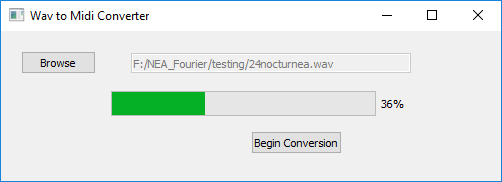
\includegraphics[width=0.9\textwidth]{Capture.PNG}
	\caption{The GUI for Running the Converter}
	\centering
\end{figure}

\begin{table}[H]
\begin{tabular}{|l|l|l|}
\hline
\textbf{Function Name} & \textbf{Inputs} & \textbf{Description}                                                                                                                                                                                                                                                                \\ \hline
\_\_init\_\_           & None            & This creates the GUI window.                                                                                                                                                                                                                                                        \\ \hline
get\_files             & None            & \begin{tabular}[c]{@{}l@{}}This opens a file explorer window and\\ returns the path of the file they select.\end{tabular}                                                                                                                                                           \\ \hline
begin                  & None            & \begin{tabular}[c]{@{}l@{}}This begins the process of converting the\\ file once the button has been clicked and\\ displays a predicted time of completion. \\ The actual conversion is handled on a \\ different thread to the GUI, to allow it\\ access to more RAM.\end{tabular} \\ \hline
main                   & A path          & \begin{tabular}[c]{@{}l@{}}This handles the actual conversion itself, \\ the different Wave, Midi and Fourier\\ objects are all created and managed here.\end{tabular}                                                                                                              \\ \hline
\end{tabular}
\end{table}

\subsection*{Algorithms and Functions}
\addcontentsline{toc}{subsection}{Algorithms and Functions}

\subsubsection*{Fourier Transform}
\addcontentsline{toc}{subsubsection}{Fourier Transform}

As mentioned, the backbone of this project relies on the Fast Fourier Transform. In order to make use of this I have implemented the Cooley-Tukey algorithm that I described in my analysis section.The flowchart for this algorithm can be seen in Figure \ref{fft_flow} and the psuedocode for this can be seen as Algorithm 2, it makes use of recursion in order to simplify the problem and turn it into something that is much easier to compute. I have implemented this in my code with the use of my custom Matrix classes.

One key point to understand is that the DFT simply represents the method of applying the Fourier Transform shown in Equation \ref{eq:Fourier_Transform} to a discrete set of data and is simply a mathematical function, whereas an FFT is a family of algorithms that speed up this process significantly. In this project I have used the Cooley-Tukey algorithm as my FFT and how this works is shown both in the flowchart in Figure \ref{fft_flow} and in Algorithm \ref{fft_algo}. Algorithm \ref{dft_algo} shows how the formula for the DFT is applied to a sample containing vector using matrix multiplication, this is taken from the form shown in Equation \ref{eq:Discrete_Fourier_Transform_Matrix}.

\begin{algorithm}
\caption{Discrete Fourier Transform}\label{dft_algo}
\begin{algorithmic}[1]

\Procedure{DFT}{vector}
\State $\textit{N} \gets \text{length of } \textit{vector}$
\State $\textit{omegaN} \gets e^{-2 \pi i / N}$
\State $\textit{matrixDFT} \gets \text{blank } \textit{N} \text{ by }\textit{N} \text{ sized matrix}$
\For {$x \gets 0, 1, 2, .., (N-1)$}
   \For {$y \gets 0, 1, 2, .., (N-1)$}
       \State $\textit{matrixDFT}[y][x] \gets \textit{omegaN}^{x*y}$
   \EndFor
\EndFor
\Return $\textit{matrixDFT} * \textit{vector}$
\EndProcedure 
\end{algorithmic}
\end{algorithm}

\begin{figure}[H]
	\centering
	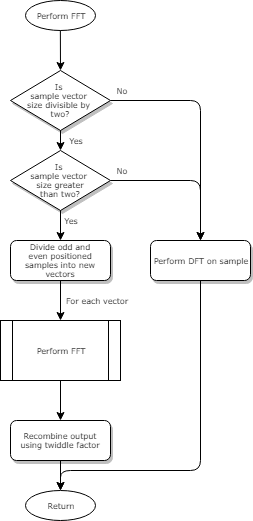
\includegraphics[width=0.65\textwidth]{flow_2.png}
	\caption{FFT Flowchart}\label{fft_flow}
	\centering
\end{figure}

\begin{algorithm}
\caption{Fast Fourier Transform}\label{fft_algo}
\begin{algorithmic}[1]
\Procedure{FFT}{vector}
\State $\textit{N} \gets \text{length of }\textit{vector}$
\If {$\textit{N} <= 2$} 
\Return DFT(\textit{vector})
\Else
\State $\textit{even} \gets \text{even positioned values of }\textit{vector}$
\State $\textit{odd} \gets \text{even positioned values of }\textit{vector}$
\State $\textit{even} \gets \text{FFT}(\textit{even})$
\State $\textit{odd} \gets \text{FFT}(\textit{odd})$
\State $\textit{powers} \gets \text{Matrix}(\text{0, 1, 2, .., \textit{N}-1})$
\State $\textit{factor} \gets -2 \pi i / N  \text{ to the power of each element of \textit{powers}} $
\State $\textit{firstHalf} \gets \text{blank \textit{N} / 2 by 1 sized matrix}$
\State $\textit{secondHalf} \gets \text{blank \textit{N} / 2 by 1 sized matrix}$
\For {$i \gets 0, 1, 2, .., N/2 $}
\State $\textit{firstHalf}[i] \gets \textit{even}[i] + \textit{odd}[i] * \textit{factor}[i]$
\State $\textit{secondHalf}[i] \gets \textit{even}[i] + \textit{odd}[i] * \textit{factor}[N/2 +i]$
\EndFor
\Return $\text{concatenation of \textit{secondHalf} onto \textit{firstHalf}}$
\EndIf
\EndProcedure
\end{algorithmic}
\end{algorithm}

To better understand this, an example of the output of this algorithm can be seen below. Figure \ref{graph_in} shows the input to the function in green, this comprises to two sine waves of different frequencies added together. When passed into the Fourier transform it is decomposed into the second function shown in Figure \ref{graph_out1}. As you can see the Fourier transform has produced two peaks, as the wave it was passed was composed of two different frequencies. The location of these peaks do not exactly match the frequencies of the original wave however, as it depends on the sampling rate of the audio where the peaks show up. In order to get the actual frequency of the wave (in Hz) out, the below formula (Formula \ref{eq:bin_to_hertz}) must be used for conversion:

\begin{equation}
    \textit{frequency in Hz} = \frac{\textit{samplerate}}{\textit{size of sample}} * \frac{\textit{bin number}}{2}
    \label{eq:bin_to_hertz}
\end{equation}


\begin{figure}[H]
	\centering
    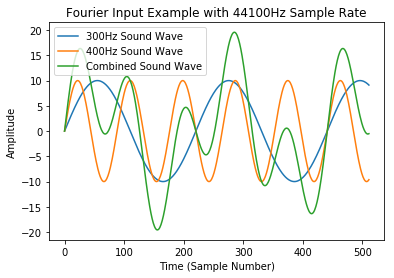
\includegraphics[width=0.85\textwidth]{input.png}
	\caption{Input Wave}\label{graph_in}
	\centering
\end{figure}

\begin{figure}[H]
	\centering
    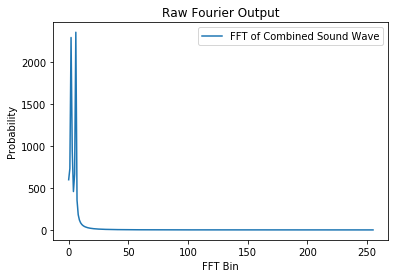
\includegraphics[width=0.85\textwidth]{output_raw.png}
	\caption{FFT Output}\label{graph_out1}
	\centering
\end{figure}


\subsubsection*{Median Filter}
\addcontentsline{toc}{subsubsection}{Median Filter}
A median filter is used on the raw results from the FFT in order to help smooth out any smaller peaks due to signal noise, this then helps with identifying the positions of peak frequencies as there is a lesser chance of false positives. A median filter works by sliding a odd-length sized window across the data and replacing the middle value with the median of the numbers in the window. The psuedocode for this can be seen below in Algorithm \ref{med_algo}.

\begin{algorithm}
\caption{Median Filter}\label{med_algo}
\begin{algorithmic}[3]

\Procedure{Median Filter}{vector, size}
\State $\textit{N} \gets \text{length of }\textit{vector}$
\State $\textit{output} \gets \text{blank \textit{N} by 1 sized matrix}$
\State $\textit{output}[0][0] \gets \textit{vector}[0][0]$
\State $\textit{output}[N-1][0] \gets \textit{vector}[N-1][0]$
\State $\textit{end} \gets \textit{size}/2$
\For {$i \gets 0, 1, .., (N-end)-size$}
    \State $\textit{window} \gets \text{\textit{vector} positions \textit{i}  to \textit{i}  + \textit{size}}/2$
    \State $\textit{output}[\textit{end}+\textit{i}][0] \gets \text{median of \textit{vector}}$
\EndFor
\Return $\textit{output}$
\EndProcedure
\end{algorithmic}
\end{algorithm}

As an example, if passed in the list [0, 3, 2, 6, 4, 0, 12, 21, 8, 0, 0, 22, 24, 26, 0, 30, 32, 0, 54, 38] with a window size of 3, then the output would be [0, 2, 3, 4, 4, 4, 12, 12, 8, 0, 0, 22, 24, 24, 26, 30, 0, 0, 0, 38]. The smoothing that this provides can be seen in the plots overleaf.

\begin{figure}[H]
	\centering
    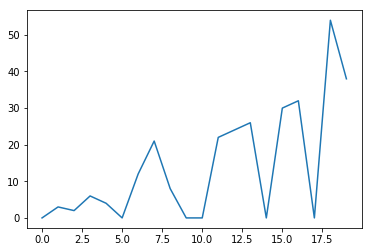
\includegraphics[width=0.85\textwidth]{med_graph_in.png}
	\caption{Input List of Random Numbers}\label{med_graph_in}
	\centering
\end{figure}

\begin{figure}[H]
	\centering
    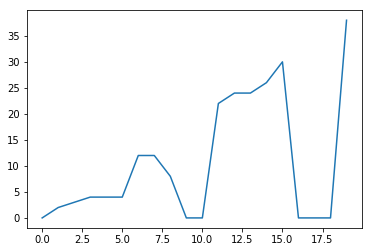
\includegraphics[width=0.85\textwidth]{med_graph_out.png}
	\caption{Output List After Median Filter}\label{med_graph_out}
	\centering
\end{figure}

\subsubsection*{Blackman-Harris Window}
\addcontentsline{toc}{subsubsection}{Blackman-Harris Window}
Windowing is a signal processing technique whereby only specific sections of data are processed at a time. For example in the median function algorithm a square window is used to look through the input vector, this involves simply looking through and taking the section of data as-is to be processed. A square window is the most simple kind of window as no further processing is required to make one, it is also sufficient for most applications such as finding a median. However with an FFT the results can be improved by using a more complicated windowing function such as the Blackman-Harris as it puts more emphasis on data towards the middle of the window. Using the Blackman-Harris the final conversion does noticeably improve in quality as it is more easily able to distinguish low-frequency notes from signal noise.

The formula for this window function can be seen below in Figure \ref{bm_form}, each value in the raw window is multiplied by the result of this function, where N is its position in the window. The result of applying this function to a window of 1s can also be seen in Figure \ref{bm_plot}.

\begin{figure}[H]
	\centering
    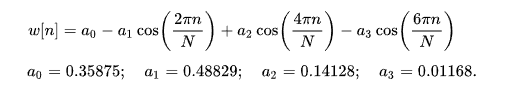
\includegraphics[width=0.9\textwidth]{blackman_harris.png}
	\caption{Blackman-Harris Function Formula}\label{bm_form}
	\centering
\end{figure}

\begin{figure}[H]
	\centering
    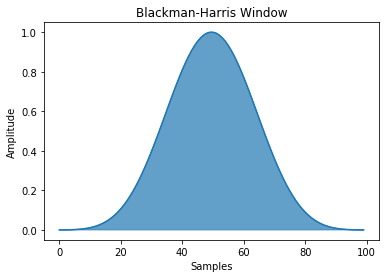
\includegraphics[width=0.9\textwidth]{blackman_harris.PNG}
	\caption{Blackman-Harris Plot}\label{bm_plot}
	\centering
\end{figure}

\subsubsection*{Peak Finding Algorithm}
\addcontentsline{toc}{subsubsection}{Peak Finding Algorithm}
In order to find all of the peaks in my FFT output I've implemented a peak-finding algorithm. This algorithm will look through the values presented and signal that there is a peak in the data when the new value it sees is more than a certain threshold away from the data it has already seen, with a prioritisation of more recent data points. This algorithm is quite robust and allows for fine-tuning of the different threshold values so I was able to set it up to work best with the data I would be feeding it. Interestingly, the origin of this algorithm was not a scientific paper or something similar, but instead an answer on StackOverflow and can be found here \textit{https://stackoverflow.com/questions/22583391/peak-signal-detection-in-realtime-timeseries-data/22640362\#22640362}.

\begin{algorithm}
\caption{Peak Finding Algorithm}\label{peak_algo}
\begin{algorithmic}[4]

\Procedure{Find Peaks}{vector, lag, threshold, influence}
\State $\textit{N} \gets \text{length of }\textit{vector}$
\State $\textit{signals} \gets \text{blank }\textit{N} \text{ by 1 matrix }$
\State $\textit{filteredY} \gets \textit{vector}$
\State $\textit{avgFilter} \gets \text{blank }\textit{N} \text{ by 1 matrix }$
\State $\textit{stdFilter} \gets \text{blank }\textit{N} \text{ by 1 matrix }$
\State $\textit{avgFilter}[lag-1] \gets \text{average of the first }\textit{lag-1} \text{ items in } \textit{vector}$
\State $\textit{stdFilter}[lag-1] \gets \text{standard deviation of the first }\textit{lag-1} \text{ items in } \textit{vector}$
\For {$i \gets (lag+1), .., (N-1)$}
    \If{$|(\textit{vector}[i][0] - \textit{avgFilter}[i-1][0])| > \textit{threshold} * \textit{stdFilter}[i-1][0]$}
        \If{$\textit{vector}[i][0] > \textit{avgFilter}[i-1][0]$}
            \State $\textit{signals}[i][0] \gets \text{1}$
        \Else
            \State $\textit{signals}[i][0] \gets \text{-1}$
        \EndIf
        \State $\textit{filteredY}[i][0] \gets \textit{influence } * \textit{vector} [i][0] + (1-\textit{influence})*\textit{filteredY}[i-1][0]$
    \Else
        \State $\textit{signals}[i][0] \gets \text{0}$
        \State $\textit{filteredY}[i][0] \gets \textit{vector}[i][0]$
    \EndIf
        \State $\textit{avgFilter}[i][0] \gets \text{the average of } \textit{filteredY} \text{ from i-lag to i}$
        \State $\textit{stdFilter}[i][0] \gets \text{the standard deviation of } \textit{filteredY} \text{ from i-lag to i}$
\EndFor
\Return $\textit{signals}$
\EndProcedure
\end{algorithmic}
\end{algorithm}

\subsection*{Postprocessing Example Output}
\addcontentsline{toc}{subsection}{Postprocessing Example Output}
When these extra algorithms are used in conjunction with the FFT, a more clear result can be obtained. For example when provided with the same input wave as shown in Figure \ref{graph_in} on page 19, the difference in outputs can be seen below as \ref{graph_out2}. The Blackman-Harris window removes some of the smoothing of the raw Fourier output, allowing a computer to more easily determine the peaks in the data.

\textbf{\begin{figure}[H]
	\centering
    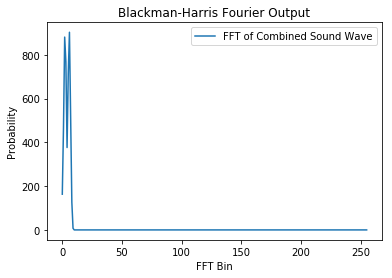
\includegraphics[width=0.9\textwidth]{output_bh.png}
	\caption{FFT Output with Blackman-Harris}\label{graph_out2}
	\centering
\end{figure}}

In order to then determine the frequency from this I use the peak finding algorithm. In order to try and identify any chords in the recording, I must look for when there are two different peaks that are not multiples of each other. This is again hard to achieve as algorithmically determining the difference between a chord and noise in the FFT result is very difficult.

\subsection*{Final Overview}
\addcontentsline{toc}{subsection}{Final Overview}
Using all of the above algorithms my program should be able to successfully complete its task of converting a wave file to a midi file. Once the samples have been read in, they will first be iterated over to determine the boundaries between where there is and is not a note. Then each section will be put through a Blackman-Harris window to better represent the frequencies that will be heard, before finally being Fast Fourier Transformed. A median filter will then be used to smooth out the results and then a peak finding algorithm used to determine the peaks. The position of these will finally be converted into a midi note and then written as a midi event to a file.

\section*{Technical Solution}
\addcontentsline{toc}{section}{Technical Solution}

\subsection*{Reference}
\addcontentsline{toc}{subsection}{Reference}

The below table shows where key features of the program are located in the program. All line numbers refer to the first file \textit{classes.py}, as \textit{gui.py} simply holds the code to run the classes and to display the GUI.

\begin{table}[H]
\begin{tabular}{|l|l|l|}
\hline
{\ul \textbf{Feature}}     & {\ul \textbf{Line Number}} & {\ul \textbf{Page Number}} \\ \hline
Matrix Multiplication      & 137                        & 37                         \\ \hline
Wave File Reading          & 291                        & 42                         \\ \hline
Discrete Fourier Transform & 423                        & 46                         \\ \hline
Peak Finding Algorithm     & 433                        & 46                         \\ \hline
Fast Fourier Transform     & 486                        & 48                         \\ \hline
Blackman-Harris Window     & 512                        & 49                         \\ \hline
Median Filter              & 534                        & 49                         \\ \hline
Midi File Writing          & 581                        & 51                         \\ \hline
\end{tabular}
\end{table}



\subsection*{classes.py}
\addcontentsline{toc}{subsection}{classes.py}
\inputminted[linenos, breaklines]{python}{code/classes.py}

\subsection*{gui.py}
\addcontentsline{toc}{subsection}{gui.py}
\inputminted[linenos, breaklines]{python}{code/gui.py}

\section*{Testing}
\addcontentsline{toc}{section}{Testing}
In order to ensure the functionality on my program I will test different aspects of its performance against my original specification. Throughout the development process I have been testing the functionality of my program using an agile programming paradigm, to ensure that each stage of the conversion process could be used to verify the next was working correctly. I have broken down the testing documentation into the components of the program of which they test.

\subsection*{The Matrix Class}
\addcontentsline{toc}{subsection}{The Matrix Class}
The tests on the Matrix class are to ensure that Objective 3 has been met by the program, to recap this means the program must be able to correctly add, multiply, slice and concatenate matrices together.

\subsubsection*{Addition}
\addcontentsline{toc}{subsubsection}{Addition}
To test the addition function I will try 3 different input cases, one with positive integers, one with a mix of positive and negative integers and one with complex numbers. The class should be able to handle a matrix containing any object types that support addition, but these 3 combinations will be encountered during the run of the program. I have also included a test to ensure the program will not attempt to perform addition on matrices of different dimensions. \\

\textbf{Test 1, Input and Expected Output}
\begin{align*}
    \begin{bmatrix} 
        1 & 2 \\
        3 & 4
    \end{bmatrix} + 
    \begin{bmatrix} 
        1 & 1 \\
        1 & 1
    \end{bmatrix} = 
    \begin{bmatrix} 
        2 & 3 \\
        4 & 5
    \end{bmatrix}
\end{align*}

\textbf{\begin{figure}[H]
	\centering
    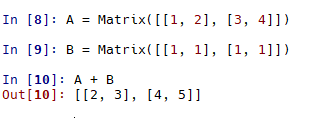
\includegraphics[width=0.9\textwidth]{tests/mat_add_1.PNG}
	\caption{Test 1, Success}
	\centering
\end{figure}}

\textbf{Test 2, Input and Expected Output}
\begin{align*}
    \begin{bmatrix} 
        1 & 2 \\
        3 & 4
    \end{bmatrix} + 
    \begin{bmatrix} 
        -1 & -2 \\
        -4 & -3
    \end{bmatrix} = 
    \begin{bmatrix} 
        0 & 0 \\
        -1 & 1
    \end{bmatrix}
\end{align*}

\textbf{\begin{figure}[H]
	\centering
    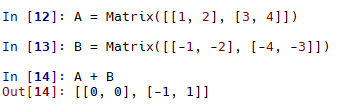
\includegraphics[width=0.9\textwidth]{tests/mat_add_2.PNG}
	\caption{Test 2, Success}
	\centering
\end{figure}}

\textbf{Test 3, Input and Expected Output}
\begin{align*}
    \begin{bmatrix} 
        1 & 2 \\
        3 & 4
    \end{bmatrix} + 
    \begin{bmatrix} 
        i & -2i \\
        -1 & 2
    \end{bmatrix} = 
    \begin{bmatrix} 
        1+i & 2-2i \\
        2 & 6
    \end{bmatrix}
\end{align*}

\textbf{\begin{figure}[H]
	\centering
    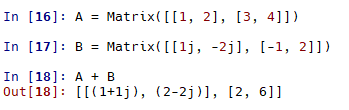
\includegraphics[width=0.9\textwidth]{tests/mat_add_3.PNG}
	\caption{Test 3, Success}
	\centering
\end{figure}}

\textbf{Test 4, Input and Expected Output}
\begin{align*}
    \begin{bmatrix} 
        1 \\
        2
    \end{bmatrix} + 
    \begin{bmatrix} 
        1 & 1 \\
        1 & 1
    \end{bmatrix} = 
    ERROR
\end{align*}

\textbf{\begin{figure}[H]
	\centering
    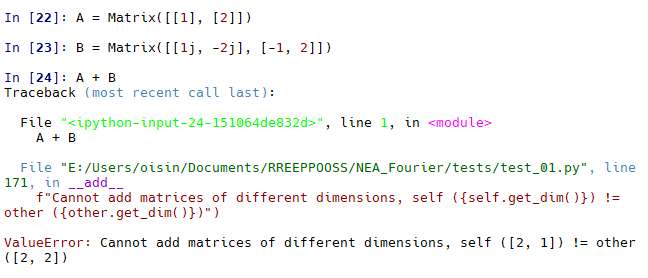
\includegraphics[width=0.9\textwidth]{tests/mat_add_4.PNG}
	\caption{Test 4, Success}
	\centering
\end{figure}}

\subsubsection*{Multiplication}
\addcontentsline{toc}{subsubsection}{Multiplication}
To test the multiplication functionality, I need to ensure that the class can handle all types of multiplication between vectors, scalars and matrices correctly. Some combinations of matrix multiplication are not mathematically valid, so I need to ensure my program correctly determines when it can and cannot perform a multiplication.\\

\textbf{Test 1, Input and Expected Output}
\begin{align*}
    \begin{bmatrix} 
        1 & 2 \\
        3 & 4
    \end{bmatrix}
    \begin{bmatrix} 
        1 & 1 \\
        1 & 1
    \end{bmatrix} = 
    \begin{bmatrix} 
        3 & 3 \\
        7 & 7
    \end{bmatrix}
\end{align*}

\textbf{\begin{figure}[H]
	\centering
    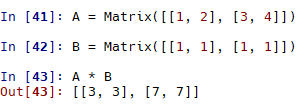
\includegraphics[width=0.9\textwidth]{tests/mat_mul_1.PNG}
	\caption{Test 1, Success}
	\centering
\end{figure}}

\textbf{Test 2, Input and Expected Output}
\begin{align*}
    \begin{bmatrix} 
        1 & 1 \\
        1 & 1
    \end{bmatrix}
    \begin{bmatrix} 
        1 & 2 \\
        3 & 4
    \end{bmatrix} = 
    \begin{bmatrix} 
        4 & 6 \\
        4 & 6
    \end{bmatrix}
\end{align*}

\textbf{\begin{figure}[H]
	\centering
    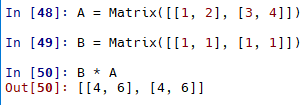
\includegraphics[width=0.9\textwidth]{tests/mat_mul_2.PNG}
	\caption{Test 2, Success}
	\centering
\end{figure}}

\textbf{Test 3, Input and Expected Output}
\begin{align*}
    \begin{bmatrix} 
        1 & 2 \\
        3 & 4
    \end{bmatrix}
    \begin{bmatrix} 
        2\\
        4
    \end{bmatrix} = 
    \begin{bmatrix} 
        10\\
        22
    \end{bmatrix}
\end{align*}

\textbf{\begin{figure}[H]
	\centering
    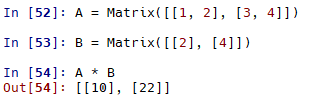
\includegraphics[width=0.9\textwidth]{tests/mat_mul_3.PNG}
	\caption{Test 3, Success}
	\centering
\end{figure}}

\textbf{Test 4, Input and Expected Output}
\begin{align*}
    \begin{bmatrix} 
        2\\
        4
    \end{bmatrix}
    \begin{bmatrix} 
        1 & 2 \\
        3 & 4
    \end{bmatrix} = 
    ERROR
\end{align*}

\textbf{\begin{figure}[H]
	\centering
    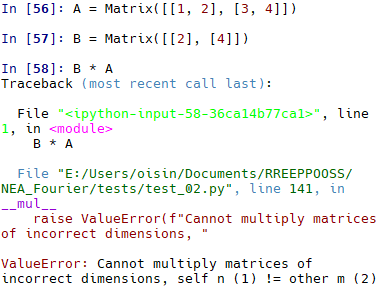
\includegraphics[width=0.9\textwidth]{tests/mat_mul_4.PNG}
	\caption{Test 4, Success}
	\centering
\end{figure}}

\textbf{Test 5, Input and Expected Output}
\begin{align*}
    3
    \begin{bmatrix} 
        1 & 2 \\
        3 & 4
    \end{bmatrix} =
    \begin{bmatrix} 
        3 & 6 \\
        9 & 12
    \end{bmatrix}
\end{align*}

\textbf{\begin{figure}[H]
	\centering
    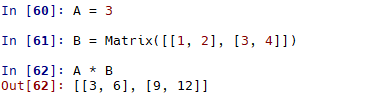
\includegraphics[width=0.9\textwidth]{tests/mat_mul_5.PNG}
	\caption{Test 5, Success}
	\centering
\end{figure}}

\subsubsection*{Slicing}
\addcontentsline{toc}{subsubsection}{Slicing}

\textbf{Test 1, Input and Expected Output}
\begin{align*}
    \begin{bmatrix} 
        1 & 2 & 3\\
        4 & 5 & 6\\
        7 & 8 & 9
    \end{bmatrix}
    .section( 1, 1, "vertical")
    ->
    \begin{bmatrix} 
        2 \\
        5 \\
        8
    \end{bmatrix}
\end{align*}

\textbf{\begin{figure}[H]
	\centering
    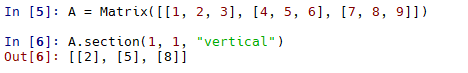
\includegraphics[width=0.9\textwidth]{tests/mat_sli_1.PNG}
	\caption{Test 1, Success}
	\centering
\end{figure}}

\textbf{Test 2, Input and Expected Output}
\begin{align*}
    \begin{bmatrix} 
        1 & 2 & 3\\
        4 & 5 & 6\\
        7 & 8 & 9
    \end{bmatrix}
    .section( 1, 5, "vertical")
    ->
    \begin{bmatrix} 
        2 & 3\\
        5 & 6\\
        8 & 9
    \end{bmatrix}
\end{align*}

\textbf{\begin{figure}[H]
	\centering
    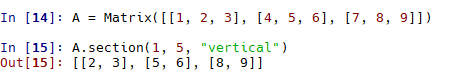
\includegraphics[width=0.9\textwidth]{tests/mat_sli_2.PNG}
	\caption{Test 2, Success}
	\centering
\end{figure}}

\textbf{Test 3, Input and Expected Output}
\begin{align*}
    \begin{bmatrix} 
        1 & 2 & 3\\
        4 & 5 & 6\\
        7 & 8 & 9
    \end{bmatrix}
    .section( 1, 2, "horizontal")
    ->
\begin{bmatrix} 
        4 & 5 & 6\\
        7 & 8 & 9
    \end{bmatrix}
\end{align*}

\textbf{\begin{figure}[H]
	\centering
    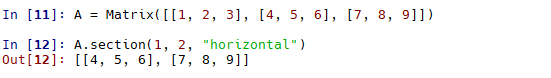
\includegraphics[width=0.9\textwidth]{tests/mat_sli_3.PNG}
	\caption{Test 3, Success}
	\centering
\end{figure}}

\subsubsection*{Concatenation}
\addcontentsline{toc}{subsubsection}{Concatenation}

\textbf{Test 1, Input and Expected Output}
\begin{align*}
    \begin{bmatrix} 
        1 & 2 \\
        3 & 4
    \end{bmatrix}.concatenate(
    \begin{bmatrix} 
        1 & 1 \\
        1 & 1
    \end{bmatrix}, "vertical") -> 
    \begin{bmatrix} 
        1 & 2 \\
        3 & 4 \\
        1 & 1 \\
        1 & 1
    \end{bmatrix}
\end{align*}

\textbf{\begin{figure}[H]
	\centering
    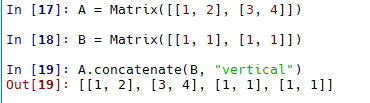
\includegraphics[width=0.9\textwidth]{tests/mat_cat_1.PNG}
	\caption{Test 1, Success}
	\centering
\end{figure}}

\textbf{Test 2, Input and Expected Output}
\begin{align*}
    \begin{bmatrix} 
        1 & 2 \\
        3 & 4
    \end{bmatrix}.concatenate(
    \begin{bmatrix} 
        1 \\
        1
    \end{bmatrix}, "horizontal") -> 
    \begin{bmatrix} 
        1 & 2 & 1\\
        3 & 4 & 1
    \end{bmatrix}
\end{align*}

\textbf{\begin{figure}[H]
	\centering
    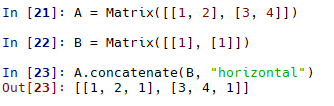
\includegraphics[width=0.9\textwidth]{tests/mat_cat_2.PNG}
	\caption{Test 2, Success}
	\centering
\end{figure}}

\textbf{Test 3, Input and Expected Output}
\begin{align*}
    \begin{bmatrix} 
        1 & 2 \\
        3 & 4
    \end{bmatrix}.concatenate(
    \begin{bmatrix} 
        1 \\
        1
    \end{bmatrix}, "vertical") -> 
    ERROR
\end{align*}

\textbf{\begin{figure}[H]
	\centering
    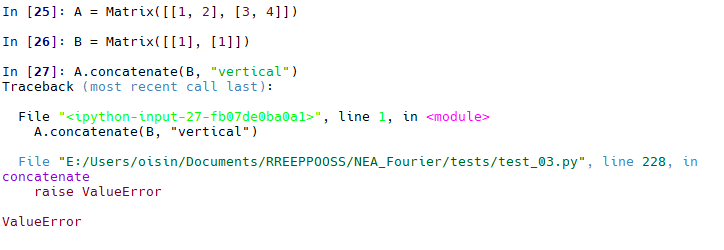
\includegraphics[width=0.9\textwidth]{tests/mat_cat_3.PNG}
	\caption{Test 3, Success}
	\centering
\end{figure}}

\subsection*{The Wave Class}
\addcontentsline{toc}{subsection}{The Wave Class}
The wave class only performs the task of reading in a file to begin with, but to do this it makes use of several methods that need to be tested. In order to test the overall result of this is correct, the wave file is opened using a program called audacity to view the raw waveform.

\textbf{Test 1, Input and Expected Output}
The input was a wave recording of 3 blind mice, which can be heard in the testing video (link on page 76).

\textbf{\begin{figure}[H]
	\centering
    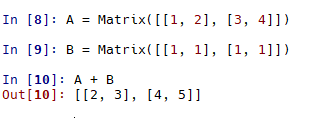
\includegraphics[width=0.9\textwidth]{tests/mat_add_1.PNG}
	\caption{Test 1, Success}
	\centering
\end{figure}}

\subsection*{The Fourier Class}
\addcontentsline{toc}{subsection}{The Fourier Class}
This class is the most important to the success of the project, so ensuring it worked correctly was a top priority. Both the FFT and DFT should produce the same results for the same input, but for large inputs the FFT will be faster. 

\textbf{Test 1, Input and Expected Output}
\begin{align*}
    DFT(
    \begin{bmatrix} 
        1\\
        0\\
        0\\
        0\\
        0\\
        0\\
        0\\
        0
    \end{bmatrix})
    ->
    \begin{bmatrix} 
        1\\
        1\\
        1\\
        1\\
        1\\
        1\\
        1\\
        1
    \end{bmatrix}
\end{align*}

\textbf{\begin{figure}[H]
	\centering
    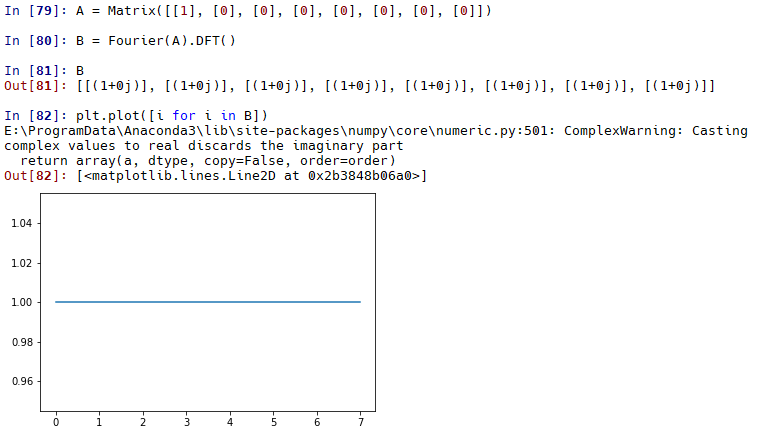
\includegraphics[width=0.9\textwidth]{tests/fourier_1.PNG}
	\caption{Test 1, Success}
	\centering
\end{figure}}

\textbf{Test 2, Input and Expected Output}
\begin{align*}
    DFT(
    \begin{bmatrix} 
        0\\
        1\\
        0\\
        0\\
        0\\
        0\\
        0\\
        0
    \end{bmatrix})
    ->
    \begin{bmatrix} 
        1\\
        7.07-7.07i\\
        0-i\\
        -7.07-7.07i\\
        -1\\
        -7.07+7.07i\\
        0+i\\
        7.07+7.07i
    \end{bmatrix}
\end{align*}

\textbf{\begin{figure}[H]
	\centering
    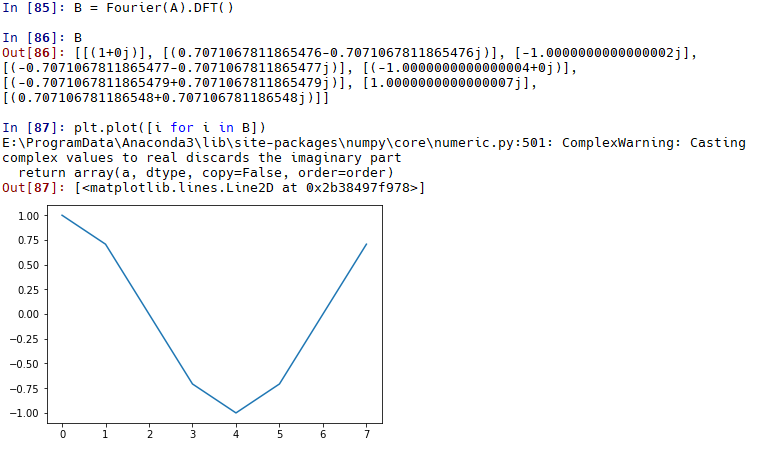
\includegraphics[width=0.9\textwidth]{tests/fourier_2.PNG}
	\caption{Test 2, Success}
	\centering
\end{figure}}

\textbf{Test 3, Input and Expected Output}
\begin{align*}
    FFT(
    \begin{bmatrix} 
        1\\
        0\\
        0\\
        0\\
        0\\
        0\\
        0\\
        0
    \end{bmatrix})
    ->
    \begin{bmatrix} 
        1\\
        1\\
        1\\
        1\\
        1\\
        1\\
        1\\
        1
    \end{bmatrix}
\end{align*}

\textbf{\begin{figure}[H]
	\centering
    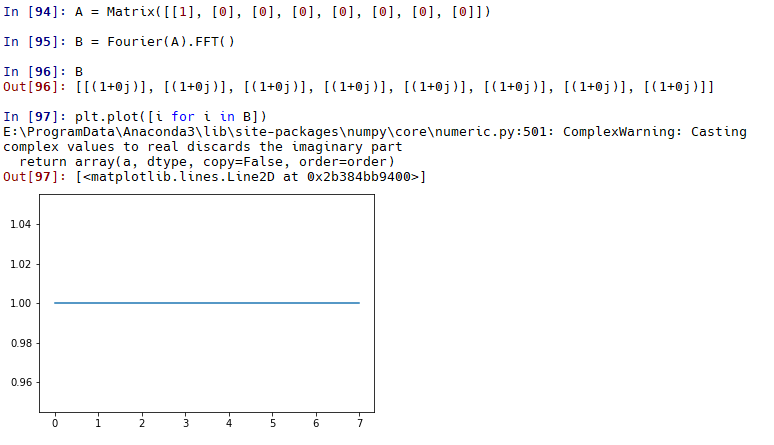
\includegraphics[width=0.9\textwidth]{tests/fourier_3.PNG}
	\caption{Test 3, Success}
	\centering
\end{figure}}

\textbf{Test 4, Input and Expected Output}
\begin{align*}
    FFT(
    \begin{bmatrix} 
        0\\
        1\\
        0\\
        0\\
        0\\
        0\\
        0\\
        0
    \end{bmatrix})
    ->
    \begin{bmatrix} 
        1\\
        7.07-7.07i\\
        0-i\\
        -7.07-7.07i\\
        -1\\
        -7.07+7.07i\\
        0+i\\
        7.07+7.07i
    \end{bmatrix}
\end{align*}

\textbf{\begin{figure}[H]
	\centering
    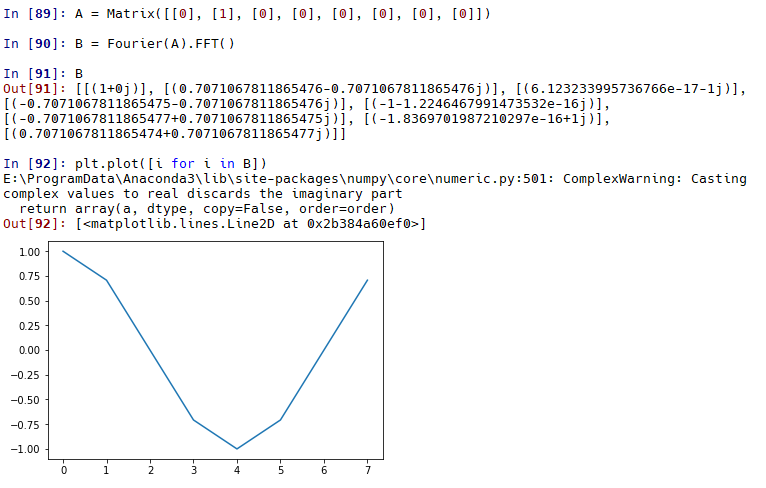
\includegraphics[width=0.9\textwidth]{tests/fourier_4.PNG}
	\caption{Test 4, Success}
	\centering
\end{figure}}


\subsection*{The Midi Class}
\addcontentsline{toc}{subsection}{The Midi Class}
The midi class writes the final file out to disk, so it needs to always correctly format the output file to ensure that it is readable by any synthesizer the user wants to use to play back the file.

\textbf{Test 1, Input and Expected Output}
By inputting the results of the conversion of the 3 Blind Mice file, the midi class should write a correctly formatted file to disk.

\textbf{\begin{figure}[H]
	\centering
    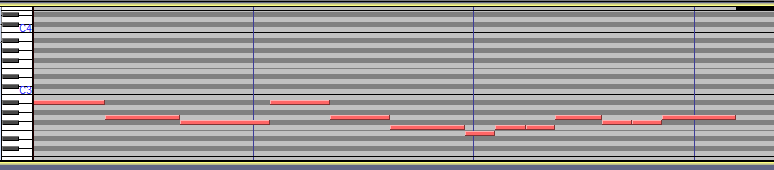
\includegraphics[width=0.9\textwidth]{tests/midi_1.PNG}
	\caption{Test 1, Success}
	\centering
\end{figure}}

\subsection*{The GUI Class}
\addcontentsline{toc}{subsection}{The GUI Class}
The GUI itself is quite simple, as there are few options for the user to configure. The main features are the time estimation, progress bar and the ability to queue up files.

\textbf{Test 1, Input and Expected Output}
The GUI should launch.

\textbf{\begin{figure}[H]
	\centering
    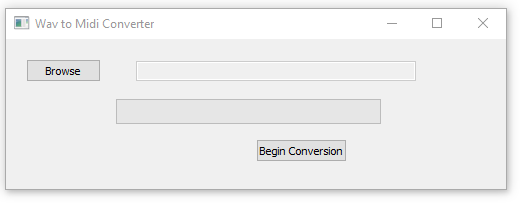
\includegraphics[width=0.9\textwidth]{tests/GUI_1.PNG}
	\caption{Test 1, Success}
	\centering
\end{figure}}

\textbf{Test 2, Input and Expected Output}
When clicked, the browse button should open a file explorer window allowing the user to select a file.

\textbf{\begin{figure}[H]
	\centering
    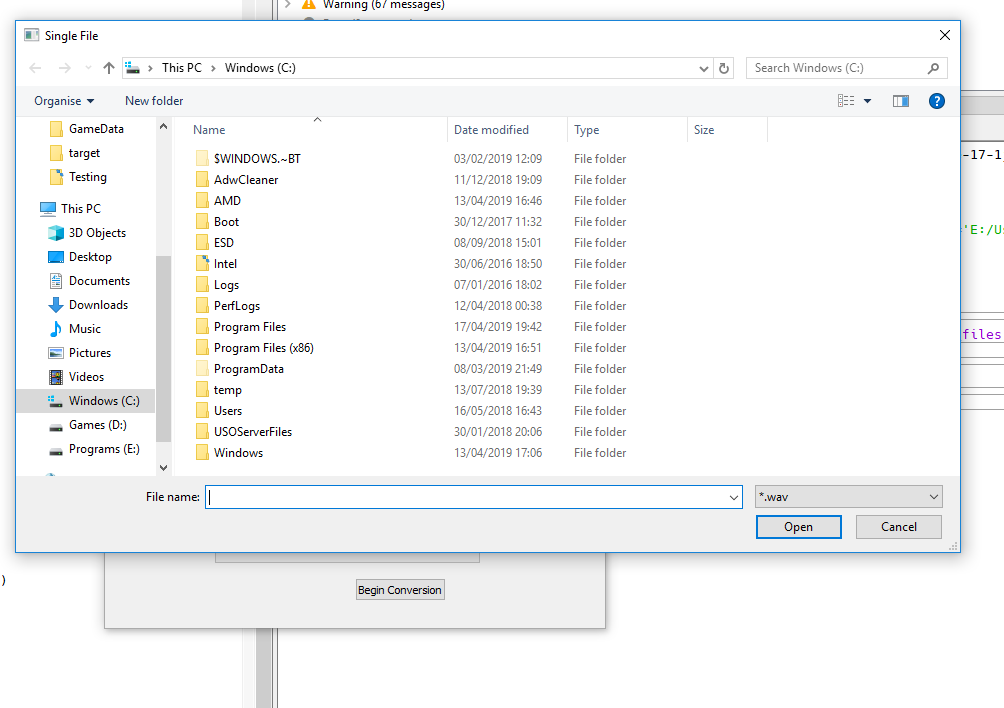
\includegraphics[width=0.9\textwidth]{tests/GUI_2.PNG}
	\caption{Test 2, Success}
	\centering
\end{figure}}

\textbf{Test 3, Input and Expected Output}
Before conversion, a popup should appear with an estimated length of time until the conversion is completed. This time is a slight overestimate and represents a worse case scenario. 

\textbf{\begin{figure}[H]
	\centering
    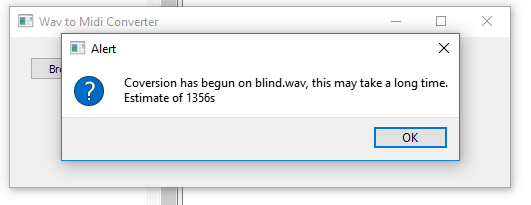
\includegraphics[width=0.9\textwidth]{tests/GUI_3.PNG}
	\caption{Test 3, Success}
	\centering
\end{figure}}

\textbf{Test 4, Input and Expected Output}
During a conversion a progress bar should be shown to the user, this should update as the conversion progresses.

\textbf{\begin{figure}[H]
	\centering
    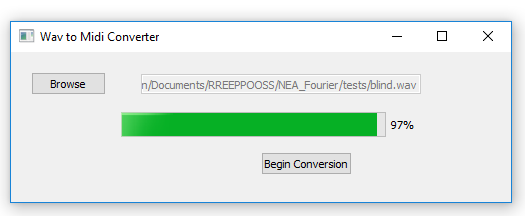
\includegraphics[width=0.9\textwidth]{tests/GUI_4.PNG}
	\caption{Test 4, Success}
	\centering
\end{figure}}

\subsection*{The Complete Solution}
\addcontentsline{toc}{subsection}{The Complete Solution}
As the result of this program is an audio file instead of visual, I have created several recordings of the program operating to showcase this. Each of the files that can be found in the following Google Drive folder \textit{https://youtu.be/9qqKU9sJCDg} contains a video walking through the tests and their outcomes. In summary however the program performs as expected in all areas, the final quality of the conversion were not as good as the online Bear converter however. I believe this was due to not using autocorrelation, although it may have been other factors. Despite this however, the program has still met its objectives as I did not expect the conversion to be perfect. In addition feedback from the end user describes the final result as good enough for their purposes, no converter can be 100\% accurate but I am overall pleased at how mine turned out.

\section*{Evaluation}
\addcontentsline{toc}{section}{Evaluation}
In conclusion my solution does solve the problem that it set out to do. Whilst it is not as fast or accurate as the online solution provided by Bear, it does fulfil the needs of my user by running offline and having the code publicly available and editable so it was a success.

\subsection*{Objective Completion}
\addcontentsline{toc}{subsection}{Objective Completion}
All objectives set out in my Analysis section were successfully completed, no objectives that I set out to fulfil based on the needs of my user were left incomplete. Of the extension tasks, one was completed allowing for the user to queue multiple files when using the GUI. The velocity of notes was partially implemented, however this feature is disabled by default as it did not add a noticeable change to the audio quality whilst still increasing compute time.

\begin{enumerate}
    \item The program must be able to read the samples from a wave file into an object that represents the samples and information of the file. - This has been completed as required, any type of wave file can be read in for conversion.
    \item The program must be able to perform the matrix operations:
    \begin{enumerate}
        \item Addition - Complete
        \item Multiplication - Complete
        \item Slicing - Complete
        \item Concatenation - Complete
    \end{enumerate}
    \item The program must be able to correctly write the results to a midi file, providing the input file is under a length of 3 minutes. - This has been completed, with a file size greater than 3 minutes long the program can become unstable although this happens somewhat randomly. By staying below the 3 minute mark the performance is much more consistent. 
    \item The user must be able to select a wave file to convert using a GUI. - Complete, as mentioned files can also be queued.
    \item The user must be able to select a wave file to convert without using a GUI. - Complete
    \item The user must receive conformation that the conversion has taken place successfully, or that an error of some kind has occurred. - Complete, a series of notification boxes ran on separate threads will alert the user if anything has gone wrong.
    \item During conversion, the user should have visual feedback in the form of a timer or progress bar to ensure the program is functioning. - Complete
    \item The program must be able to convert files that have only one note played at a time. - Complete
\end{enumerate}

\subsection*{End User Feedback}
\addcontentsline{toc}{subsection}{End User Feedback}
After showcasing my final solution to both the end user interviewed in my Analysis and one of their friends I am pleased with the responses that they had to it. I was happy to see that they thought it met their needs enough that they could use it when required and that the accuracy was good enough for this as well. The program's UI was simple enough that they needed no instruction on how to use the program and they especially liked the inclusion of the progress bar. They did mention that the speed would be a prime area for improvement although it was not a major issue as they were able to queue up multiple songs to be converted overnight or whilst they were working on something else. Overall the feedback has been positive.

\subsection*{Further Work}
\addcontentsline{toc}{subsection}{Further Work}
As this topic still represents a fairly open problem, an almost endless amount of optimisation could be performed on the code to increase its accuracy and speed. In particular there are two main areas I would like to expand upon, these being the use of autocorrelation and the speed of the program. Theoretically autocorrelation should yield much better results than the "pure" FFT that I am currently using, although I could not get it working to do so with the time available, so it would be interesting to spend more time and implement that successfully. I would also like to try porting the codebase into a different language, such as Java or MATLAB to try and improve the efficiency of it. Python has allowed me to rapidly prototype and develop my solution, but it is unideal for running performance critical code as it cannot be compiled and is relatively optimised for it. Further optimisation could likely be made in the existing Python codebase, although I am unsure how effective they could be versus the time required to implement them. By far the most complex and time-consuming part of this project has been the research and understanding required to solve the problem, so with this now out of the way I could probably start in another language and implement a better second version much more rapidly.

%-=------------------------------------------------------------------------------
% REFERENCES
%-------------------------------------------------------------------------------

\newpage
\addcontentsline{toc}{section}{Bibliography}
\begin{thebibliography}{9}


\bibitem{Ableton} 
Ableton Music Editor
\\\texttt{https://www.ableton.com/en/manual/converting-audio-to-midi/}

\bibitem{Wavesum} 
Wavemid Converter
\\\texttt{http://wavesum.net/wavemid-audio-to-midi.html}

\bibitem{Widisoft} 
Widisoft Music Processing Package
\\\texttt{https://www.widisoft.com/english/mp3-midi-products.html}

\bibitem{MIDI1} 
The Taiwan National University, The Midi File Format
\\\texttt{https://www.csie.ntu.edu.tw/~r92092/ref/midi/}

\bibitem{MIDI2} 
Center for Computer Assisted Research in the Humanities 
at Stanford University, The MIDI Standard
\\\texttt{http://www.ccarh.org/courses/253/handout/smf/}

\bibitem{Wave} 
Unknown Stanford Unvirsity Website
\\\texttt{http://soundfile.sapp.org/doc/WaveFormat/}

\bibitem{FFT} 
NTI Audio, Fast Fourier Transform FFT
\\\texttt{https://www.nti-audio.com/en/support/know-how/fast-fourier-transform-fft}

\bibitem{gauss} 
Gauss, Carl Friedrich (1876)
\\\texttt{Theoria Interpolationis Methodo Nova Tractata, page 265-327}

\bibitem{spectrum} 
G. Heinzel, A. Rudiger, and R. Schilling, Max Planck Society (2002)
\\\texttt{Spectrum and spectral density estimation by the discrete fourier
transform (DFT), including a comprehensive list of window functions and some new at-top windows}

\bibitem{autocorrelation_transcription} 
Giuliano Monti, Mark Sandler, Department of Electronic Engineering, King's College London (2000)
\\\texttt{MONOPHONIC TRANSCRIPTION WITH AUTOCORRELATION}

\bibitem{pitch_detection} 
Lizhe Tan and Montri Karnjanadecha, Prince of Songkla University (2003)
\\\texttt{PITCH DETECTION ALGORITHM : AUTOCORRELATION METHOD AND AMDF}

\bibitem{pitch_perception} 
William A. Yost, Arizona State University (2009)
\\\texttt{Pitch Perception}

\bibitem{w_k} 
L. Cohen (1998)
\\\texttt{The generalization of the Wiener-Khinchin theorem}

\bibitem{cooley} 
Cooley, James W.; Tukey, John W. (1965)
\\\texttt{An algorithm for the machine calculation of complex Fourier series}

\end{thebibliography}
\textbf{All web links were accessed and correct as of April 2019}
\end{document}




%-------------------------------------------------------------------------------
% SNIPPETS
%-------------------------------------------------------------------------------

%\begin{figure}[!ht]
%	\centering
%	\includegraphics[width=0.8\textwidth]{file_name}
%	\caption{}
%	\centering
%	\label{label:file_name}
%\end{figure}

%\begin{figure}[!ht]
%	\centering
%	\includegraphics[width=0.8\textwidth]{graph}
%	\caption{Blood pressure ranges and associated level of hypertension (American Heart Association, 2013).}
%	\centering
%	\label{label:graph}
%\end{figure}

%\begin{wrapfigure}{r}{0.30\textwidth}
%	\vspace{-40pt}
%	\begin{center}
%		\includegraphics[width=0.29\textwidth]{file_name}
%	\end{center}
%	\vspace{-20pt}
%	\caption{}
%	\label{label:file_name}
%\end{wrapfigure}

%\begin{wrapfigure}{r}{0.45\textwidth}
%	\begin{center}
%		\includegraphics[width=0.29\textwidth]{manometer}
%	\end{center}
%	\caption{Aneroid sphygmomanometer with stethoscope (Medicalexpo, 2012).}
%	\label{label:manometer}
%\end{wrapfigure}

%\begin{table}[!ht]\footnotesize
%	\centering
%	\begin{tabular}{cccccc}
%	\toprule
%	\multicolumn{2}{c} {Pearson's correlation test} & \multicolumn{4}{c} {Independent t-test} \\
%	\midrule	
%	\multicolumn{2}{c} {Gender} & \multicolumn{2}{c} {Activity level} & \multicolumn{2}{c} {Gender} \\
%	\midrule
%	Males & Females & 1st level & 6th level & Males & Females \\
%	\midrule
%	\multicolumn{2}{c} {BMI vs. SP} & \multicolumn{2}{c} {Systolic pressure} & \multicolumn{2}{c} {Systolic Pressure} \\
%	\multicolumn{2}{c} {BMI vs. DP} & \multicolumn{2}{c} {Diastolic pressure} & \multicolumn{2}{c} {Diastolic pressure} \\
%	\multicolumn{2}{c} {BMI vs. MAP} & \multicolumn{2}{c} {MAP} & \multicolumn{2}{c} {MAP} \\
%	\multicolumn{2}{c} {W:H ratio vs. SP} & \multicolumn{2}{c} {BMI} & \multicolumn{2}{c} {BMI} \\
%	\multicolumn{2}{c} {W:H ratio vs. DP} & \multicolumn{2}{c} {W:H ratio} & \multicolumn{2}{c} {W:H ratio} \\
%	\multicolumn{2}{c} {W:H ratio vs. MAP} & \multicolumn{2}{c} {\% Body fat} & \multicolumn{2}{c} {\% Body fat} \\
%	\multicolumn{2}{c} {} & \multicolumn{2}{c} {Height} & \multicolumn{2}{c} {Height} \\
%	\multicolumn{2}{c} {} & \multicolumn{2}{c} {Weight} & \multicolumn{2}{c} {Weight} \\
%	\multicolumn{2}{c} {} & \multicolumn{2}{c} {Heart rate} & \multicolumn{2}{c} {Heart rate} \\
%	\bottomrule
%	\end{tabular}
%	\caption{Parameters that were analysed and related statistical test performed for current study. BMI - body mass index; SP - systolic pressure; DP - diastolic pressure; MAP - mean arterial pressure; W:H ratio - waist to hip ratio.}
%	\label{label:tests}
%\end{table}